\documentclass{book}
\usepackage{amsmath}
\usepackage{amsthm}
\usepackage{amsfonts}
\usepackage{mathrsfs}
\usepackage{chngcntr}
\usepackage{bm}
\usepackage[usenames,dvipsnames]{xcolor}
\usepackage{tikz}
\usetikzlibrary{patterns}
\usepackage{hyperref}

\hypersetup{
    colorlinks,
    linkcolor={red!30!black},
    citecolor={blue!50!black},
    urlcolor={blue!80!black}
}

\renewcommand{\thechapter}{\Roman{chapter}}
\makeatletter
  \renewcommand\l@chapter{\@dottedtocline{2}{1.5em}{2.5em}}
  \renewcommand\l@section{\@dottedtocline{2}{2.5em}{3.5em}}
\makeatother

\numberwithin{equation}{section}
\renewcommand{\theequation}{\textbf{\arabic{section}}.\arabic{equation}}

\theoremstyle{plain}
\newtheorem{thm}{Theorem}
\newtheorem{lem}[thm]{Lemma}
\newtheorem{prop}{Proposition}
\newtheorem{cor}{Corollary}

\theoremstyle{definition}
\newtheorem{defn}{Definition}[section]

\theoremstyle{remark}
\newtheorem{rem}{Remark}

\makeatletter
\newtheoremstyle{BoldStyle}
  {6pt}% space before
  {6pt}% space after
  {%\addtolength{\@totalleftmargin}{3.5em}
   %\addtolength{\linewidth}{-3.5em}
   %\parshape 1 3.5em \linewidth
  }% body font
  {}% indent
  {\bf }% header font
  {.}% punctuation
  {.3em}% after theorem header
  {}% header specification (empty for default)
\makeatother

\theoremstyle{BoldStyle}

\newtheorem{exercise}{Exercise}
\newtheorem*{exercise*}{Exercise}
\numberwithin{exercise}{section}

\definecolor{DarkBlue}{RGB}{0,0,64}
\definecolor{DarkBrown}{RGB}{64,20,10}
\definecolor{DarkGreen}{RGB}{0,64,0}
\definecolor{DarkPurple}{RGB}{64,0,42}

% annotation macros
\newcommand{\repl}[2]{{\color{gray} [#1] }{\color{blue} #2}}
\newcommand{\add}[1]{{\color{blue} #1}}
\newcommand{\del}[1]{{\color{gray} [#1]}}
\newcommand{\note}[1]{{\color{DarkGreen}\footnotesize \textsc{Note.} #1}}
\newcommand{\answer}[1]{{\color{DarkBlue}\footnotesize \textsc{Answer.} #1}}
\newcommand{\solution}[2]{{\color{DarkBlue}\footnotesize \textsc{Solution #1.} #2}}
\newcommand{\summary}[1]{{\color{DarkPurple}\footnotesize \textsc{Summary.} #1}}


\begin{document}


\title{Notes on \emph{Stochastic Process in Physics and Chemistry}\cite{vankampen}}
\author{N. G. Van Kampen}
\date{3rd Edition (May 7, 2007)}

\maketitle

\tableofcontents


\chapter{Stochastic Variables}

\section{Definition}

\begin{defn}
  A continuous \emph{probability distribution}
  (\emph{probability density}) is a function
  that satisfies
  \begin{equation}
    P(x) \ge 0
    \label{eq:Px_nonneg}
  \end{equation}
  and
  \begin{equation}
    \int P(x) \, dx = 1.
    \label{eq:Px_normalize}
  \end{equation}
\end{defn}

For a mixture of discrete and continuous distribution,
\begin{equation}
  P(x) = \sum_n p_n \, \delta(x - x_n) + \tilde P(x).
  \label{eq:Px_mixture}
\end{equation}

The normalization is
$$
\sum_{n} p_n + \int \tilde P(x) \, dx = 1.
$$

\subsection*{Excursus}

\begin{defn}
  The \emph{cumulative distribution function}
  (\emph{probability distribution function})
  is defined as
  \begin{equation}
    \mathbb{P}(x) = \int_{-\infty}^{x+0} P(x') \, dx'.
  \end{equation}
\end{defn}

\paragraph{Axiomatic probability theory.}

References\cite{kolmogorov}.

\begin{enumerate}
\item The $x$-axis $\rightarrow$ a set $S$.
\item An interval $dx$ $\rightarrow$ a subset $A \subset S$.
\item Each subset $A$ is assigned
  a nonnegative number $\mathcal P(A)$, such that
  $$
  \mathcal P(S) = 1.
  $$
  For disjoint $A$ and $B$,
  $$
  \mathcal P(A + B) = \mathcal P(A) + \mathcal P(B).
  $$
  This is called the \emph{probability measure}.
\end{enumerate}

\begin{exercise*}
{\bf Rencontre problem (Matching problem).}
%
What's the probability that an arbitrary permutation
of $n$ objects leaves no object in its place?
%
Using the hint, we have
$$
n \, p(n) - (n-1) \, p(n-1) = p(n-2).
$$

Then
$$
n \, [p(n) - p(n-1)] = - [ p(n-1) - p(n-2)].
$$
and
$$
p(n) - p(n-1) = \frac{ (-1)^{n} }{n!}.
$$
So
$$
p(n) = \sum_{i = 0}^n \frac{ (-)^{k} } { k! } \rightarrow e^{-1}.
$$

\end{exercise*}


\section{Averages}

Given a distribution $P(X)$, the average of $f(X)$ is computed by
$$
\langle f(X) \rangle
=
\int f(x) \, P(x) \, dx.
$$

A most commonly-used average is the $m$-th moment:
$$
\mu_m = \langle X^m \rangle.
$$
Here, $\mu_1$ is the mean, and
\begin{equation}
\sigma^2 =
\left\langle
  (X - \langle X \rangle )^2
\right\rangle
= \mu_2 - \mu_1^2,
\end{equation}
is the variance, and $\sigma$ is the standard deviation.

An interesting observation is that
not all probability distributions have a finite variance.
%
A famous example is the Lorentz distribution
\begin{equation}
P(x) = \frac{1}{\pi} \frac{\gamma}{ (x-a)^2 + \gamma^2 },
\qquad (-\infty < x < \infty).
\end{equation}


\begin{exercise}
For the \emph{square distribution},
\begin{equation}
P(x) =
\begin{cases}
  0,          \qquad &\mathrm{for\;} |x| > a, \\
  (2a)^{-1},  \qquad &\mathrm{for\;} |x| < a. \\
\end{cases}
\end{equation}
We have $\mu_{2n+1} = 0$, and
$$
\mu^{2n}
=
\int_{-a}^a \frac{x^{2n}}{2a} \, dx
=
\frac{ a^{2n} }{ 2n + 1 }.
$$
\end{exercise}

\begin{exercise}
For the \emph{Gauss distribution},
\begin{equation}
  P(x) = (2 \pi)^{-\frac 1 2} e^{-\frac{1}{2} x^2}.
\end{equation}
We have
$$
\begin{aligned}
  \mu_{2n+1} &= 0, \\
  \mu_{2n}  &= (2n-1)!!.
\end{aligned}
$$
\end{exercise}

\begin{exercise}
Find a distribution whose moments $\mu_n$ exists up to but not beyond a prescribed $n$.

The answer is
$$
P(x) = \frac{ \alpha } { (x^2 + 1)^{1 + \frac{n}{2} } }.
$$
The normalization $\alpha$ is determined as follows.
$$
\begin{aligned}
1 &= \int_{-\infty}^\infty P(x) \, dx
  = \alpha \int_{-\pi/2}^{\pi/2} \frac{ \sec^2\theta } { \sec^{n+2}\theta } \, d\theta
  =\alpha \int_{-\pi/2}^{\pi/2} \cos^n\theta \, d\theta
  = B\left(\frac{n+1}{2}, \frac{1}{2}\right).
\end{aligned}
$$
So
$$
\alpha = \frac{ \Gamma(\frac n  2 + 1) } { \Gamma(\frac{n+1}{2}) \, \Gamma(\frac 1 2) }
=
\begin{cases}
  \frac{n!!}{(n-1)!! }\frac{1}{\pi}, & n \mathrm{\; is \; even} \\
  \frac{n!!}{(n-1)!! }\frac{1}{2}, & n \mathrm{\; is \; odd}
\end{cases}
$$
\end{exercise}

\begin{exercise}
From
$$
f = \langle
|\lambda_0 + \lambda_1 \, X + \cdots + \lambda_n \, X^n|^2 \rangle \ge 0,
$$
we have
$$
\mathbf \Lambda^T
\left(
  \begin{array}{ccccc}
    1     & \mu_1 & \dots & \mu_n \\
    \mu_1 & \mu_2 & \dots & \mu_{n+1} \\
    \vdots& \vdots&       & \vdots \\
    \mu_n &\mu_{n+1}&\dots& \mu_{2n}
  \end{array}
\right)
\mathbf \Lambda
\ge 0.
$$
Since $\Lambda = (\lambda_0, \dots, \lambda_n)^T$ is arbitrary,
the matrix in the middle is nonnegative-definite,
meaning that every eigenvalue is nonnegative,
so is their product, or the determinant.
$$
\left|
  \begin{array}{ccccc}
    1     & \mu_1 & \dots & \mu_n \\
    \mu_1 & \mu_2 & \dots & \mu_{n+1} \\
    \vdots& \vdots&       & \vdots \\
    \mu_n &\mu_{n+1}&\dots& \mu_{2n}
  \end{array}
\right| \ge 0
$$
\end{exercise}


\begin{exercise}
Eq. \eqref{eq:Px_nonneg} can be replaced with the condition
$$
\int f(x) P(x) \, dx \ge 0,
$$
for any continuous $f(x)$.
\end{exercise}


\begin{exercise}
Show that for $n = 1, 2, 3, \dots$,
$$
P(x) = n \frac{e^{-x}}{x} I_n(x),
$$
has no average.

Notes.
$$
e^{ \frac{x}{2} \left( t + \frac{1}{t} \right) }
= \sum_{n = -\infty}^\infty I_n(x) \, t^n.
$$
And
$$
I_n(x) = \sum_{r = 0}^\infty \frac{1}{r! (r + n)!} \left(\frac x 2\right)^{n+2r}.
$$
\end{exercise}



\subsection*{Characteristic function}

\begin{defn}
The \emph{characteristic function} is defined as
\begin{equation}
G(k) = \langle e^{ikX} \rangle
=
\int e^{ikx} P(x) \, dx.
\end{equation}
\end{defn}

The characteristic function satisfies
\begin{equation}
  G(0) = 1, \qquad
  |G(k)| \le 1.
\end{equation}


The characteristic function is also the \emph{moment generating function}
because
\begin{equation}
  G(k) = \sum_{k = 0}^\infty \frac{(tk)^m } {m!} \mu_m.
  \label{eq:mugen}
\end{equation}
Similarly $\log G(k)$
\begin{equation}
  \log G(k) = \sum_{k = 0}^\infty \frac{(tk)^m } {m!} \kappa_m,
  \label{eq:kappagen}
\end{equation}
is the generating function of cumulants $\kappa_m$.
The first few are listed below.
\begin{equation}
  \begin{aligned}
    \kappa_1 &= \mu_1, \\
    \kappa_2 &= \mu_2 - \mu_1^2, \\
    \kappa_3 &= \mu_3 -3 \, \mu_2 \, \mu_1 + 2 \, \mu_1^3, \\
    \kappa_4 &= \mu_4 -4 \, \mu_3 \, \mu_1 - 3 \, \mu_2^2 + 12 \, \mu_2 \, \mu_1^2 - 6 \, \mu_1^4.
  \end{aligned}
\end{equation}


\section{Multivariate distributions}

\section{Addition of stochastic variables}

\section{Transformation of variables}

\section{The Gaussian distribution}

\section{The central limit theorem}




\chapter{Random Events}

\section{Definition}

\section{The Poisson distribution}

\section{Alternative description of random events}

\section{The inverse formula}

\section{The correlation functions}

\section{Waiting times}

\section{Factorial correlation functions}


\chapter{Stochastic Processes}

\section{Definition}

\section{Stochastic process in physics}

\section{Fourier transformation of stationary process}

\section{The hierarchy of distribution functions}

\paragraph{Stationary Process.}

A process is \emph{stationary} if all $P_n$ depend on the time difference alone.

$$
P_n(y_1, t_1 + \tau; y_2, t_2 + \tau; \cdots; y_n, t_n + \tau)
=
P_n(y_1, t_1; y_2, t_2; \cdots; y_n, t_n).
$$


\paragraph{Gaussian process.}

a process is \emph{Gaussian} if all $P_n$ are
(multivariate) Gaussian distributions.


\section{The vibrating string and random fields}

\section{Branching process}


\chapter{Markov Processes}


\section{Markov property}

\section{The Chapman-Kolmogorov equation}

Page 78.
A Markov process:
$$
P_{1|n-1}(y_n, t_n| y_1, t_1; \dots, y_{n-1}, t_{n-1})
=
P_{1|1}(y_n, t_n|y_{n-1},t_{n-1})
$$
where, $P_{1|1}$ is the transition probability.

Page 79.
Wiener process (Wiener-L\'evy process)
\begin{equation}
P_{1|1}(y_2, t_2|y_1, t_1)
=
\frac{1}{\sqrt{2\,\pi(t_2 - t_1)}}
\exp\left[
  -\frac{ (y_2 - y_1)^2 } { 2 \, (t_2 - t_1) }
\right].
\tag{2.4}
\end{equation}
%
\begin{equation}
P_1(y, t)
=
\frac{1}{\sqrt{2\,\pi\,t}}
\exp\left[
  -\frac{ y^2 } { 2 \, t }
\right].
\tag{2.5}
\end{equation}


Page 80.
Poisson process
\begin{equation}
P_{1|1}(n_2, t_2|n_1, t_1)
=
\frac{ (t_2 - t_1)^{n_2 - n_1} } { (n_2 - n_1)! }
e^{ -(t_2 - t_1) },
\tag{2.6}
\end{equation}
where
$P_1(n, 0) = \delta_{n,0}$.

Page 81. Ex. 5 Eq. (2.8)

$$
\frac{ \partial P } { \partial t }
=
D \frac{ \partial^2 P } { \partial y^2 }.
$$
Show (2.5) satisfies this by $D = \frac{1}{2}$.
Generally, try
$$
P = \frac{ 1 } { \sqrt{ 2 \, \pi \, a(t) } }
\exp\left(
  - \frac{ y^2 } { 2 \, a(t) }
\right).
$$
Then,
$$
\begin{aligned}
\frac{ \partial P } { \partial y }
&=
- \frac{ y } { a } P
\\
\frac{ \partial^2 P } { \partial y^2 }
&=
- \frac{1}{a} P
+ \frac{ y^2 } { a^2 } P
\\
\frac{ \partial P } { \partial t }
&=
-\frac{ a' } { 2 \, a } P
+ \frac{ y^2 } { 2 \, a^2 } a' P.
\end{aligned}
$$
So $a'(t) = 2 \, D(t)$,
and
$a(t) = 2 \int^t_0 D(s) \, ds$.


\section{Stationary Markov process}

Page 83.
Ornstein-Uhlenbeck (OU) process.
Phys. Rev. 36 823 (1930).
\begin{equation}
P_1(y_1)
=
\frac{1}{\sqrt{2 \, \pi} e^{-\frac 1 2 y_1^2 } }
\tag{3.10}
\end{equation}

\begin{equation}
  T_\tau(y_2 | y_1)
=
\frac{ 1 } { \sqrt{ 2 \, \pi \, (1 - e^{-2\tau}) }  }
\exp\left[
  -\frac{ (y_2 - y_1 e^{-\tau})^2 }
  { 2 ( 1 - e^{-2 \tau } ) }
\right]
\tag{3.11}
\end{equation}

Page 84.
Doob's theorem.
J. L. Doob Annals of Math. 43, 351 (1942).

If a process is stationary, Gaussian and Markovian,
essential OU is the only process with these properties.

Page 85.
Exercise 8. (3.11) satisfies
\begin{align}
\frac{ \partial T } { \partial \tau }
&=
\frac{ \partial } { \partial y_2 } \left( y_2 T \right)
+
\frac{ \partial^2 T } { \partial y_2^2 }
\quad \mathrm{forward}
\tag{3.20}
\\
\frac{ \partial T } { \partial \tau }
&=
-y_1 \frac{ \partial T } { \partial y_1 }
+
\frac{ \partial^2 T } { \partial y_1^2 }
\quad \mathrm{backward}
\tag{3.21}
\end{align}


Page 86.
Exercise 12.
Cauchy process.
\begin{equation}
  T_\tau(y_2|y_1)
  =
  \frac{1}{\pi}
  \frac{ \tau } { (y_2 - y_1)^2 + \tau^2 }.
\end{equation}
Prove it satisfies Chapman-Kolmogorov.
$$
\begin{aligned}
\int T_{\tau'}(y_3|y_2) T_\tau(y_2|y_1) \, dy_2
&=
\int \int \int \tilde T_\tau \, \tilde T_\tau' \,
e^{-i(k + k') y_2 } \frac{dk}{2\pi} \frac{dk'}{2\pi} dy_2
\\
&=
\int e^{ -i|k| (\tau +\tau') + ik (y_1 -y_3) } \frac{dk}{2\pi}
\\
&=
\frac{1}{\pi}
\frac{ \tau + \tau'}
{ (\tau + \tau')^2 + (y_3 - y_1)^2 } \\
&=
T_{\tau + \tau'}(y_3 | y_1) \\
\end{aligned}
$$



\section{The extraction of a subensemble}

\section{Markov chains}

\section{The decay process}


\chapter{The Master Equation}

\section{Derivation}

For a Markov process,
the master equation is the differential equation
of the transition probabilities $T_{\tau'}$
for vanishing time difference $\tau'$.
%
In other words,
it is the zero time limit of
the Chapman-Kolmogorov equation.


In the limit of small $\tau'$,
the transition probabilities $T_{\tau'}$ can be expanded as
%
\begin{equation}
  T_{\tau'}(y_2 | y_1)
  =
  \left[1 - a_0(y_1) \, \tau'\right] \, \delta(y_2 - y_1)
  +
  \tau' \, W(y_2 | y_1) + o(\tau'),
  \label{eq:transproba_smallt}
\end{equation}
%
where $W(y_2 | y_1)$ is the \emph{transition probability per unit time}
from $y_1$ to $y_2$,
and hence
%
\begin{equation}
  W(y_2 | y_1) \ge 0.
  \label{eq:W_positive}
\end{equation}
%
The coefficient $1-a_0\, \tau'$ is the probability that no transition takes place
during $\tau'$.  So
%
\begin{equation}
  a_0(y)
  =
  \int W(y_2 | y_1) \, dy_2.
  \label{eq:total_W}
\end{equation}
%
This also follows from $T_{\tau'}(y_2 | y_1) \, dy_2 = 1$.



Now the Chapman-Kolmogorov equation is
\begin{equation}
  T_{\tau' + \tau}(y_3 | y_1)
  =
  \int T_{\tau'}(y_3 | y_2) \, T_\tau(y_2 | y_1) \, dy_2,
  \tag{IV.3.2}
  \label{eq:ChapmanKolmogorov}
\end{equation}
which means in this case (expanding $T_{\tau'}$ but not $T_\tau$)
{\footnotesize
$$
\begin{aligned}
  T_{\tau' + \tau}(y_3 | y_1)
  &=
  \int \left[1 - a_0(y) \, \tau'\right] \, \delta(y_3 - y_2) \, T_\tau(y_2 | y_1) \, dy_2
  +
  \tau' \int W(y_3|y_2) \, T_\tau(y_2 | y_1) \, dy_2
  \\
  &=
  \left[1 - a_0(y_3) \, \tau'\right] \, T_\tau(y_3 | y_1)
  +
  \tau' \int W(y_3 | y_2) \, T_\tau(y_2 | y_1) \, dy_2.
\end{aligned}
$$
}
Differentiate this equation with respect to $\tau'$,
set $\tau' \to 0$ and use \eqref{eq:total_W},
\begin{align}
\frac{ \partial } { \partial \tau } T_\tau(y_3 | y_1 )
&=
-a_0(y_3) \, T_\tau(y_3 | y_1)
+
\int W(y_3 | y_2) \, T_\tau(y_2 | y_1) \, dy_2
\notag \\
&=
\int
\left[
  W(y_3 | y_2) \, T_\tau(y_2 | y_1)
  -
  W(y_2 | y_3) \, T_\tau(y_3 | y_1)
\right] \, dy_2.
\label{eq:master_equation_T}
\end{align}
%
The differential form of the Chapman-Kolmogorov equation
is called the \emph{master equation},
or \emph{M-equation}.

The simplified, more intuitive form is
%
\begin{align}
  \frac{ \partial } { \partial t } P(y, t)
&=
\int
\left[
  W(y | y') \, P(y', t)
  -
  W(y' | y) \, P(y, t)
\right] \, dy'.
\label{eq:master_equation_continuous}
\end{align}
%
The equation describes the evolution of
the transition probability
from the initial condition $P(y, t_1) = \delta(y - y_1)$.
%
The master equation is \emph{not} meant as an equation
for the single-time distribution $P_1(y, t)$.

\paragraph{Discrete case.}

The discrete case is given by
%
\begin{equation}
\frac{ d p_n(t) } { dt }
=
\sum_{n'}
\left\{
  W_{n n'} p_{n'}(t)
  -
  W_{n' n} p_n(t)
\right\}.
\label{eq:master_equation_discrete}
\end{equation}
%
The master equation is a gain-loose equation
for the probability of discrete state $n$.
%
The first term on the right-hand side is the gain;
the second the loss;
the $n = n'$ terms do not contribute.


The elements $W_{n n'}$ of the transition matrix
can be, for example, obtained from Fermi's Golden rule:
$$
W_{n n'} = \frac{ 2 \, \pi } { \hbar } \, \left| H'_{n n'} \right| \, \rho(E_n).
$$
This formula is derived from the perturbation theory
in quantum mechanics, with
$\rho(E_n) = \left| \langle \psi | \psi \rangle \right|$.

\paragraph{Example of the decay process.}

The transition probability is
$$
T_{\Delta t}(n | n')
=
\begin{cases}
  n' \, \gamma \, \Delta t    & \mathrm{for} \; $n = n' - 1$ \\
  0   & \mathrm{otherwise.}
\end{cases}
$$
So $W_{n n'} = \gamma \, \delta_{n, n' - 1} n'$, and
\begin{equation}
\frac{ d p_n } { dt }
=
\gamma \, (n + 1) \, p_{n+1}(t)
-\gamma \, n \, p_n(t).
\label{eq:decay_master_equation}
\end{equation}
%
Consider $\langle N(t) \rangle$,
\begin{align}
  \sum_n n \dot p_n
  &=
  \sum_n \gamma \, (n + 1) \, n \, p_{n+1}(t)
  -
  \sum_n \gamma \, n^2 \, p_n(t)
  \notag \\
  &=
  \gamma \,
  \sum_n
  \left\{
    n(n-1) p_n - n^2 p_n
  \right\}
  \notag \\
  &=
  -\gamma \sum_n n \, p_n,
  \label{eq:decay_nave_diffeq1}
\end{align}
which means
\begin{equation}
  \frac{ d } { dt } \langle N(t) \rangle
  =
  -\gamma \, \langle N(t) \rangle,
  \label{eq:decay_nave_diffeq}
\end{equation}
%
and
\begin{equation}
  \langle N(t) \rangle
  =
  n_0 \, e^{-\gamma \, t}
  \label{eq:decay_nave_sol}
\end{equation}



\begin{exercise}
  Derive the M-equation for the dichotomic (2-state) Markov process.

  \answer{
  \begin{align}
  T_\tau
  &= \frac{1}{2}(1 + e^{-2\gamma \tau}) \, \delta_{y, y'}
  +\frac{1}{2}(1 - e^{-2\gamma \tau}) \, \delta_{y, -y'}
  \tag{IV.2.3}
  \label{eq:dichotomic_T}
  \\
  &\stackrel{\tau \to 0}{=\joinrel=}
  (1 - \gamma \tau) \, \delta_{y, y'} + \gamma \, \tau \, \delta_{y, -y'},
  \notag
  \end{align}
  which means $W_{y, -y} = \gamma$.
  The master equation is
  $$
  \frac{ d p_y(t) } { dt }
  = \gamma \, p_{-y}(t) - \gamma \, p_y(t).
  $$
  }
\end{exercise}


\begin{exercise}
  Solve the above equation.

  \answer{
  $$
  \frac{ d ( p_y - p_{-y} ) } { dt }
  = -2 \, \gamma \, (p_y - p_{-y} ).
  $$
  which yields
  $$
  p_y - p_{-y} = e^{-2 \, \gamma \, t} (p_y - p_{-y})\big|_{t = 0}
  = e^{-2\, \gamma \, t} (\delta_{y, y_0} - \delta_{y, -y_0}).
  $$
  On the other hand, we have
  $$
  p_y + p_{-y} = 1 = \delta_{y, y_0} + \delta_{y, -y_0}.
  $$
  Averaging the above two equations, we get
  $$
  p_y
  = \frac{1}{2}(1 + e^{-2\gamma \, t}) \, \delta_{y, y'}
  +\frac{1}{2}(1 - e^{-2\gamma \, t}) \, \delta_{y, -y'}.
  $$
  agreeing with \eqref{eq:dichotomic_T}.
  }
\end{exercise}

\begin{exercise}
  Show that the solution of \eqref{eq:decay_master_equation}
  with $p_n(0) = \delta_{n, n0}$
  must vanish for $n > n_0$ for $t \ge 0$,
  so we can truncate the sum at $n = n_0$.

  \answer{
  For $n > n_0$, the right-hand side of \eqref{eq:decay_master_equation}
  vanishes at initially, hence $dp_n/dt = 0$.
  %
  Integrating the master equation for $\Delta t$ yields $p_n(\Delta t) = 0$.
  %
  The process can be continued for $2 \Delta t, 3 \Delta t, \dots$,
  so $p_n(t) = 0$ for $t > 0$.
  }
\end{exercise}

\begin{exercise}
  Similar to \eqref{eq:decay_nave_diffeq1}, derive
  $\langle N(t)^2 \rangle$ and
  $\langle\langle N(t)^2 \rangle\rangle$.

  \answer{
    Multiplying \eqref{eq:decay_master_equation} by $n^2$
    and summing over $n$, we get
    $$
    \frac{ d } { d t } \langle N(t)^2 \rangle
    =
    \gamma \sum_{n} \left( n \, (n-1)^2 \, p_n - n^3 \, p_n \right)
    =
    - 2 \, \gamma \langle N(t)^2 \rangle
    + \gamma \langle N(t) \rangle.
    $$
    The solution is
    $$
    \langle N(t)^2 \rangle
    =
    n_0^2 \, e^{-2\,\gamma \, t}
    + \gamma \int_0^t \langle N(\tau)\rangle e^{-2\, \gamma \, (t - \tau)} d\tau
    =
    n_0^2 \, e^{-2\,\gamma \, t}
    +
    n_0 \, \left(e^{-\gamma \, t} - e^{\gamma \, t} \right).
    $$
  }
\end{exercise}

\begin{exercise}
  Solve the master equation for the Kangaroo process,
  in which $W(y|y') = u(y) \, v(y')$.

  \answer{
  The master equation becomes
  $$
  \frac{ \partial P } { \partial t }
  =
  u(y) \, \int v(y') \, P(y', t) \, dy'
  -
  \left[\int u(y') \, dy' \right]
  v(y) \, P(y, t)
  =
  u(y) \, \sigma(t) - \phi(y) \, P(y, t),
  $$
  where $\sigma(t) \equiv \int v(y) \, P(y, t) \, dy$
  and
  $\phi(y) = v(y) \int u(y') \, dy'$.
  %
  The equation can be readily solve for a fixed $y$:
  \begin{equation}
  P(y, t)
  =
  P(y, 0) \, e^{-\phi(y) \, t}
  +
  u(y) \int_0^t \sigma(\tau) \, e^{-\phi(y) \, (t - \tau)} \, d\tau.
  \label{eq:kangaroo_P}
  \end{equation}
  Multiply $v(y)$ and integrate
  $$
  \sigma(t) = \int v(y) \, P(y, 0) \, e^{-\phi(y) \, t} dy
  +
  \int u(y) \, v(y) \, dy
  \int_0^t \sigma(\tau) \, e^{-\phi(y) \, (t - \tau) } d\tau.
  $$
  Laplace transform this equation for time $t$,
  $$
  \mathcal L\sigma
  =
  \int \frac{ v(y) \, P(y, 0) \, dy } { s + \phi(y) }
  +
  \int u(y) \, v(y) \, dy \frac{ \mathcal L\sigma }{ s + \phi(y) }.
  $$
  and the solution is
  $$
  \mathcal L\sigma
  =
  \left. \int \frac{ v(y) \, P(y, 0) \, dy } { s + \phi(y) }
  \middle/
  \left[
    1 - \int \frac{ u(y) \, v(y) \, dy }{ s + \phi(y) }
  \right]
  \right..
  $$
  Using this in \eqref{eq:kangaroo_P} yields $P(y, t)$.
  }
\end{exercise}

\begin{exercise}
  Solve the case of $v = v_0$ being a constant.

  \answer{
  In this case, $\sigma(t) = v_0$,
  $\phi = v_0 \int u(y') \, dy' = \phi_0$
  is a constant,
  and
  $
  \int u(y) \sigma(\tau) e^{-\phi(y) (t - \tau)} d\tau
  = u(y) \, v_0 \, (1 - e^{-\phi_0 \, t}) / \phi_0.
  $
  So, \eqref{eq:kangaroo_P} becomes
  $$
  P(y, t)
  =
  P(y, 0) \, e^{-\phi_0 \, t}
  +
  \frac{ u(y) } { \int u(y') \, dy' }
  \left(
    1 - e^{-\phi_0 \, t}
  \right).
  $$
  The first term on the right-hand side represents
  the decay of the initial distribution;
  the second term represents the growth of the stationary distribution
  $u(y) / \int u(y') \, dy'$.
  }
\end{exercise}


% section 2
\section{Class of $\mathbb W$-matrices}

Define a matrix
\begin{equation}
  \mathbb W_{nn'} = W_{nn'} - \delta_{nn'} \left( \sum_{n''} W_{n'' n} \right).
  \label{eq:Wmatrix_discrete}
\end{equation}
%
where the second term gives the total probability loss
on the diagonals.
%
Then \eqref{eq:master_equation_discrete}
can be rewritten as
%
\begin{equation}
  \dot p_n(t) = \sum_{n'} \mathbb W_{nn'} p_n'(t).
  \label{eq:master_equation_discrete_Wmatrix}
\end{equation}
%
Or, in matrix form
%
\begin{equation}
  \dot p(t) = \mathbb W \, p(t).
  \label{eq:master_equation_discrete_Wmatrix_mat}
\end{equation}


Formally the solution is
%
\begin{equation}
  \dot p(t) = e^{t \, \mathbb W} p(0).
  \label{eq:pvec_solution}
\end{equation}
%
If detailed balance is satisfied, then $\mathbb W$ is symmetric with respect to
the stationary distribution $p^*$:
$$
\mathbb W_{n n'} p^*_{n'} = \mathbb W_{n' n} p^*_{n}.
$$
Then, a complete set of eigenvectors exists,
and \eqref{eq:master_equation_discrete_Wmatrix_mat}
can be solved by a superposition of eigensolutions.
%
For a general $\mathbb W$, this may not work.


The $\mathbb W$ matrix has two properties
\begin{equation}
  \begin{aligned}
    \mathbb W_{n n'} &\ge 0,   & \mathrm{for \;} n \ne n'; \\
    \sum_{n} \mathbb W_{n n'} &= 0 & \mathrm{for \; each \;} n
  \end{aligned}
  \label{eq:Wmatrix_properties}
\end{equation}
%
The first property follows from the non-negativity of transition probabilities;
%
the second from the balance of probabilities.
%
We say that a matrix satisfying these properties is a $\mathbb W$ matrix.

The second property of \eqref{eq:Wmatrix_properties}
means that $\mathbb W$ has a left eigenvector $\psi = (1, 1, \dots)$
with eigenvalue $0$.
%
Thus, there is at least one right eigenvector $\phi$ with the same eigenvalue.
$$
\mathbb W \, \phi = 0.
$$
If the components of $\phi$ are non-negative,
then $\phi$ represents the stationary distribution.

\note{
  If a matrix $\mathbf A$ has a left eigenvector $\psi$
  with eigenvalue $\lambda$,
  then the matrix has a right eigenvector $\phi$
  with the same eigenvalue.

  For a matrix $\mathbf A$, a right eigenvector $\phi$ satisfies
  \begin{equation}
  \left\{
    \begin{array}{ccc}
    \sum_i A_{1i} \, \phi_i = \lambda \, \phi_1 \\
    \vdots  \\
    \sum_i A_{ni} \, \phi_i = \lambda \, \phi_n
  \end{array}
  \right.
  \tag{a}
  \label{eq:right_eigenvector}
  \end{equation}
  This is a set of homogeneous equations.
  So the number of independent variables is $n - 1$,
  e.g., $\left(\phi_1/\phi_n, \dots, \phi_{n-1}/\phi_n\right)$.
  However, there are $n$ equations,
  and a solution is not guaranteed.

  If the matrix has a left vector $\psi$, such that
  $\psi \, \mathbb A = \lambda \, \psi$,
  we have
  $\psi \, \mathbb A \, \phi = \lambda \, \psi \, \phi$,
  and
  \begin{equation}
    \psi_1 \, \sum_i A_{1i} \, \phi_i
    + \dots +
    \psi_n \sum_i A_{ni} \, \phi_i
    = \lambda \, \psi_1 \, \phi_1
    + \lambda \, \psi_n \, \phi_n.
  \tag{b}
  \label{eq:left_right_eigenvectors}
  \end{equation}
  This means if the first $n-1$ equations of \eqref{eq:right_eigenvector}
  are satisfied, then the last equation is automatically satisfied
  by equation \eqref{eq:left_right_eigenvectors}.
}


$\mathbb W$ is \emph{completely reducible} or \emph{decomposable}
if by a suitable simultaneous permutation of rows and columns,
it can be cast into th form
%
\begin{equation}
  \mathbb W
  =
  \left(
  \begin{array}{ccc}
    \mathbb A   &     0     \\
    0           & \mathbb B
  \end{array}
  \right)
  \label{eq:W_decomposable}
\end{equation}
%
here $\mathbb A$ and $\mathbb B$ are also $\mathbb W$ matrices,
and they represent two macro states with no transitions in between.
%
If the eigenvectors with zero eigenvalues are $\phi^A$ and $\phi^B$,
we have two linearly independent eigenvectors
%
\begin{equation*}
  \left(
    \begin{array}{ccc}
      \mathbb A   &     0 \\
      0           & \mathbb B
    \end{array}
  \right)
  \left(
    \begin{array}{ccc}
      \phi^A \\
      0
    \end{array}
  \right)
  = 0,
  \qquad
  \left(
    \begin{array}{ccc}
      \mathbb A   &     0 \\
      0           & \mathbb B
    \end{array}
  \right)
  \left(
    \begin{array}{ccc}
      0 \\
      \phi^B
    \end{array}
  \right)
  = 0.
\end{equation*}
%
This means two non-interacting systems.
%


\paragraph*{Example.}

A nontrivial example is a system in which transitions conserve energy.
Each energy shell $E$ has its own M-equation,
with stationary distribution $\phi^E$.
The stationary distribution is an arbitrary linear combination.
$$
\phi = \sum_E \pi_E \, \phi^E,
$$
as long as $\pi_E \ge 0$ and $\sum_E \pi_E = 1$.
The Boltzmann distribution $\pi_E \propto \exp(-\beta \, E)$
is an example, but the only one.


A matrix is (\emph{incompletely}) \emph{reducible}
if it can be cast in the form
\begin{equation}
  \mathbb W
  =
  \left(
  \begin{array}{ccc}
    \mathbb A   & \mathbb D     \\
    0           & \mathbb B
  \end{array}
  \right)
  \label{eq:W_reducible}
\end{equation}
%
where $\mathbb A$ and $\mathbb B$ are square,
but $\mathbb D$ doesn't have to be.
%
The matrix still has an eigenvector
$\left(\begin{array}{ccc} \phi^A \\ 0 \end{array}\right)$
and
\begin{equation}
  \begin{aligned}
    \dot p_a &= \sum_{a'} \mathbb A_{a a'} p_{a'}
              + \sum_{b'} \mathbb D_{a b'} p_{b'} \\
    \dot p_b &= \sum_{b'} \mathbb B_{b b'} p_{b'}
  \end{aligned}
\end{equation}
%
Summing over $b$
$$
\frac{d}{dt} \sum_b p_b = \sum_{b'} \left( \sum_{b} \mathbb B_{b b'} \right) p_{b'}
=
-\sum_{b'} \left( \sum_{a} \mathbb D_{ab'} \right) p_{b'},
$$
which shows the states $b$ lose probability to states $a$.
%
The stationary distribution is reached only after states $b$
are depleted.
%
States $b$ are called \emph{transient}.
%
States $a$ are called \emph{absorbing}.


A $\mathbb W$ is \emph{splitting} if it can be cast into the form
%
\begin{equation}
  \mathbb W
  =
  \left(
  \begin{array}{ccc}
    \mathbb A   & 0         & \mathbb D     \\
    0           & \mathbb B & \mathbb E     \\
    0           & 0         & \mathbb C
  \end{array}
  \right),
  \label{eq:W_splitting}
\end{equation}
%
where $\mathbb A$, $\mathbb B$, and $\mathbb C$
are square $\mathbb W$ matrices,
and $\mathbb D$ and $\mathbb E$ are not completely zero.
%
The states $c$ are transient and deplete into $a$ and $b$.
%
There are at least two independent eigenvectors with eigenvalue zero
$$
  \left(
  \begin{array}{lll}
    \phi^A  \\
    0       \\
    0
  \end{array}
  \right)
  \quad
  \mathrm{and}
  \quad
  \left(
  \begin{array}{lll}
    0       \\
    \phi^B  \\
    0
  \end{array}
  \right)
$$


\begin{exercise}
  Evaluate \eqref{eq:pvec_solution}
  directly for $2 \times 2$ matrices.

  $$
    \left\{
      \begin{array}{llll}
        \mathbb W \phi_1 = 0 \\
        \mathbb W \phi_2 = \lambda_2 \phi_2
      \end{array}
    \right.
    \qquad
    \to
    \qquad
    \left\{
      \begin{array}{llll}
        e^{t \, \mathbb W} \phi_1 = \phi_1 \\
        e^{\mathbb W} \phi_2 = e^{t \, \lambda_2} \phi_2
      \end{array}
    \right.
  $$
  If $p(0) = c_1 \, \phi_1 + c_2 \, \phi_2$, then $c_1$ has to be one,
  and $p(t) = \phi_1 + e^{t \, \lambda_2} c_2 \, \phi_2$.

  Particularly, for the dichotomic process,
  $\mathbb W = \gamma \left(
    \begin{array}{llll}
        -1 & 1 \\
        1 & -1
    \end{array}\right)$,
  $\lambda_2 = -2 \, \gamma$,
  $\phi_2 = \left(
    \begin{array}{llll}
        \frac 1 2 \\
        -\frac 1 2
    \end{array}\right)$,
    and
    $p(t) =
    \left(\begin{array}{llll}
        \frac 1 2 \\
        -\frac 1 2
    \end{array}\right)
    \pm e^{-2\gamma t}
    \left(\begin{array}{llll}
        \frac 1 2 \\
        -\frac 1 2
    \end{array}\right)
    $.
\end{exercise}

\begin{exercise}
  Show that no stationary distribution for the infinite random walk
  $\dot p_n = p_{n+1} + p_{n-1} - 2 \, p_n$.

  For the stationary distribution $\dot p_n = 0$,
  and $p_{n+1} - p_{n} = p_n - p_{n-1} = a$.
  So $p_n = p_0 + n \, a$,
  and $a$ must be $0$ to ensure $p_n \ge 0 $
  for both $n \ge 0$ and $n \le 0$, then $p_0 = 1/\infty = 0$.
\end{exercise}



\chapter{One-step Processes}


\chapter{Chemical reactions}


% chapter VIII
\chapter{The Fokker-Planck Equation}

% section 1
\section{Introduction}

The Fokker-Planck equation is a master equation with
the $\mathbb W$ matrix being a 2nd-order differential operator:
%
\begin{equation}
  \frac{ \partial P(y, t) }  { \partial t }
=
-\frac{\partial } {\partial y} A(y) P
+\frac{1}{2} \frac{ \partial^2 } { \partial y^2 } B(y) P.
\label{eq:FokkerPlanck}
\end{equation}
Here the only condition is $B(y) > 0$.
Compare this to the master equation
\begin{equation}
\frac{ \partial P(y, t) } { \partial t }
=
\int \mathbb W(y, y') \, P(y', t) \, dt.
\tag{\ref{eq:FokkerPlanck}a}
\label{eq:master_W}
\end{equation}



We can break down Eq. \eqref{eq:FokkerPlanck}
to a pair of equations.
%
The first is a continuity equation
%
\begin{equation}
\frac{ \partial P(y, t) } { \partial t }
=
-\frac{ \partial J(y, t) } { \partial y },
\label{eq:FP_continuity}
\end{equation}
%
where $J(y, t)$ is the probability flux (see Figure \ref{fig:FP_continuity}),
\begin{figure}[h]
  \centering
  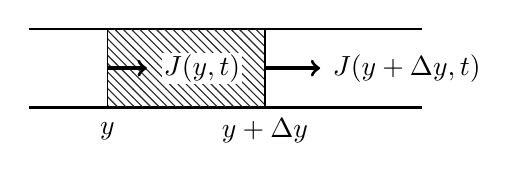
\begin{tikzpicture}
    \draw [thick]
          (0, 0) -- (5, 0)
          (0, 1) -- (5, 1);
    \draw [fill, pattern=north west lines,pattern color=black!84]
        (1, 0) -- (3, 0) -- (3, 1) -- (1, 1) -- cycle;

    \draw[very thick, ->] (1, 0.5) -- (1.5, 0.5);
    \draw[very thick, ->] (3, 0.5) -- (3.7, 0.5);

    \node[] at (1, -0.3) {$y$};
    \node[] at (3, -0.3) {$y + \Delta y$};
    \node[fill=white, inner sep=0.2mm] at (2.2, 0.5) {$J(y, t)$};
    \node[fill=white, inner sep=0.2mm] at (4.8, 0.5) {$J(y + \Delta y, t)$};
  \end{tikzpicture}
  \label{fig:FP_continuity}
  \caption{
    Continuity equation, \eqref{eq:FP_continuity}.
    $\frac{ \partial } { \partial t } \left( P \, \Delta y \right) = -J(y+ \Delta y, t) + J(y, t).$
  }
\end{figure}
%
The second is a ``constitutive equation''
%
\begin{equation}
J(y, t)
=
A(y) \, P(y, t)
-
\frac{1}{2}
\frac{ \partial }{ \partial y }
\left[
  B(y) \, P(y, t)
\right].
\label{eq:FP_constitutive}
\end{equation}
%

\note{Equation \eqref{eq:FokkerPlanck},
like the master equation,
is an equation for the transition probability
$P(y, t|y_1, t_1)$ for $t > t_1$.
%
This implies a constraint that at $t = t_1$,
$P(y, t|y_1, t_1) = \delta(y - y_1)$.
%
However, the equation is linear,
and therefore, we can use linear combination
to interpret $P(y, t)$
as the one-time probability
$P_1(y, t) \equiv \int P(y, t|y_1, t_1) \, P_1(y_1, t_1) \, dy_1$.
}

The stationary distribution is
%
\begin{equation}
  P^e(y)
  =
  \frac{ \mathrm{const.} } { B(y) }
  \exp\left[
    2 \int_0^y
      \frac{ A(y') } { B(y') } \, dy'
  \right]
  \label{eq:FP_stationary}
\end{equation}
%
provided that this distribution can be normalized.


If $A(y)$ is linear and $B(y)$ is constant,
then we can the Fokker-Planck equation is \emph{linear}:
%
\begin{equation}
  \frac{ \partial P } { \partial t }
  =
  \frac{ \partial } { \partial y }
  \left[
    (A_0 + A_1 y) \, P
  \right]
  +
  \frac{1}{2} B_0
  \frac{ \partial^2 P } { \partial y^2 }.
  \label{eq:FP_linear}
\end{equation}
%
If $A_1 < 0$,
a stationary solution exists,
and it is a Gaussian.
%
In fact,
we can turn it to the standard Ornstein-Uhlenbeck process,
%
\begin{equation}
  \frac{ \partial T }{ \partial \tau }
  =
  \frac{ \partial } { \partial y_2 }
  ( y_2 \, T )
  +
  \frac{ \partial^2 } { \partial y_2^2 } T,
  \tag{IV.3.20}
\end{equation}
%
by the following scaling
$\tau = -A_1 \, t$,
$y_2 = \sqrt{-2 \, A_1/B_0} \left(y + A_0/A_1\right)$,
and
$T = P \, (dy/dy_2) = P / \sqrt{-2 \, A_1/B_0}$.
%
So,
\emph{
  the stationary Markov process determined by
  the linear Fokker-Planck equation
  is the Ornstein-Uhlenbeck process.
}

\begin{exercise}
  Let $P(y, t|y_0, t_0)$ be solution of \eqref{eq:FokkerPlanck}.
  Take $t = t_0 + \Delta t$ and compute for small $\Delta t$
  the moments of $y - y_0 \equiv \Delta y$.
  %
  Show that for $\Delta t \to 0$
  \begin{equation}
    \frac{ \Delta y } { \Delta t }
    =
    A( y_0 ),
    \qquad
    \frac{ (\Delta y)^2 } { \Delta t }
    =
    B( y_0 ),
    \qquad
    \frac{ (\Delta y)^\nu } { \Delta t }
    =
    0 \quad (\nu \ge 3).
    \label{eq:FP_increments}
  \end{equation}

  \note{For a given model,
    \eqref{eq:FP_increments}
    serve as the standard recipe of determining
    the parameters $A(y)$ and $B(y)$
    in the Fokker-Planck equation.
  }

  \answer{
    Multiply \eqref{eq:FokkerPlanck}
    by $\Delta y^\nu$ and integrate over $y$,
    $$
    \frac{ \partial } { \partial t } \langle \Delta y^\nu \rangle
    =
    \nu \, \left\langle A(y) \Delta y^{\nu - 1} \right\rangle
    +
    \frac{1}{2} \nu \, (\nu - 1)
    \left\langle B(y) \, \Delta y^{\nu - 2} \right\rangle.
    $$
    %
    With $\nu = 1$, we get
    $$
    \frac{ \partial } { \partial t } \langle \Delta y \rangle
    =
    \langle A(y) \rangle
    \approx
    \langle A(y_0) \rangle,
    $$
    which is the first equation of \eqref{eq:FP_increments}.
    %
    Similarly, with $\nu = 2$ and $\nu \ge 3$,
    we get the second and third.
  }
\end{exercise}



\begin{exercise}
  Find the singular kernel $\mathbb W(y|y')$
  corresponding to the differential operator in \eqref{eq:FokkerPlanck}.
  %
  Calculate the jump moments (V.8.2)
  and compare the result with \eqref{eq:FP_increments}.
  [Compare (V.10.5)]


  \answer{
    The kernel is
    \begin{align}
        \mathbb W(y|y')
        &=
          -A(y') \, \delta'(y - y')
          +
          \frac 1 2
          B(y')
          \delta''(y - y')
        \tag{V.10.5} \\
        &=
        \left(
          -A(y') \frac{\partial }{\partial y }
          +
          \frac 1 2
          B(y')
          \frac{ \partial^2 } { \partial y^2 }
        \right)
        \delta(y - y')
        \tag{\ref{eq:FokkerPlanck}b}
        \label{eq:FP_Wkernel}
    \end{align}
    To verify this,
    we use this expression in \eqref{eq:master_W},
    yielding
    $$
    \frac{ \partial P } { \partial t }
    =
    -\frac{\partial }{\partial y }
    \int
      A(y')
    \delta(y - y') P(y') \, dy'
    +
    \frac 1 2
    \frac{\partial^2 }{\partial y^2 }
    \int
      B(y')
    \delta(y - y') P(y') \, dy',
    $$
    which yields \eqref{eq:FokkerPlanck}.

    For the jump moments, we have
    $$
    \begin{aligned}
    a_\nu(y')
    =
    \int (y - y')^\nu \, \mathbb W(y|y') \, dy
    =
    \int (y - y')^\nu \,
    \left(
      A(y') \frac{\partial }{\partial y' }
      +
      \frac 1 2
      B(y')
      \frac{ \partial^2 } { \partial y'^2 }
    \right)
    \delta(y - y')
    \, dy\\
    =
    -
    \int
      \frac{\partial }{\partial y' }
      \left[ (y - y')^\nu \, A(y') \right]
      \delta(y - y') \, dy
    +
      \frac 1 2
    \int
      \frac{ \partial^2 } { \partial y'^2 }
      \left[ (y - y')^\nu \, B(y') \right]
      \delta(y - y') \, dy
    .
    \end{aligned}
    $$
    Thus,
    $$
    a_1(y') = A(y') - B'(y'),
    \qquad
    a_2(y') = B(y').
    $$

    Now the expression of $a_1(y')$ contains
    an extra term $-B'(y')$,
    which is missing in the expression of \eqref{eq:FP_increments}.
    %
    Even if we average $a_1(y')$ over the distribution
    $P(y') = \delta(y' - y_0)$,
    this term would still survive.
    %
    So what went wrong?
    %
    It turns out that the expression $a_1(y')$ should really be an \emph{operator}
    instead of a number, because of the singularity of kernel $\mathbb W$.
    %
    More precisely, the $\delta''(y - y')$ in $\mathbb W$
    is defined in terms of the action on another function upon integration.
    %
    To show this, consider $I_1 = \int a_1(y') \, P(y') \, dy'$, and
    %
    $$
    \begin{aligned}
    I_1
    &=
    \int_{y'} d y' \int_y dy \, (y - y') \, \mathbb W(y|y')
    \\
    &=
    -
    \int_{y'} dy'
    \int_y
      \frac{\partial }{\partial y' }
      \left[ P(y') \, (y - y') \, A(y') \right]
      \delta(y - y') \, dy
    \\
    &\hphantom{=}
    +
      \frac 1 2
    \int_{y'} dy'
    \int_y
      \frac{ \partial^2 } { \partial y'^2 }
      \left[ P(y') \, (y - y') \, B(y') \right]
      \delta(y - y') \, dy
    \\
    &=
    \int_{y'} dy'
      P(y') \, A(y')
    -
    \int_{y'} dy'
      \frac{ \partial } { \partial y' }
      \left[ B(y') \, P(y') \right].
    \end{aligned}
    $$
    This means that $a_1(y')$ takes the operator form
    $$
    a_1(y') \equiv A(y') - \frac{d}{d y'} \left\{ B(y'), \bullet \right\},
    $$
    for which the second term always vanishes
    after integrating over another function.
  }
\end{exercise}

\begin{exercise}
  Solve \eqref{eq:FokkerPlanck} for $B(y) = 2, A(y) = -y + 1/y, y > 0$.
  Also for $B = \mathrm{constant} \ne 2$.

  \answer{We change variable to $z = y^2/2$,
    then $Q(z) = P(y) dy/dz = P(y)/y$, and \eqref{eq:FokkerPlanck}
    becomes
    $\frac{ \partial Q } { \partial t}
    = \frac{ \partial } { \partial z }
    \left[ 2 z \left(1 + \frac{ \partial } { \partial z } \right) Q \right].$
    Now consider the characteristic function
    $g = \langle e^{-sz} \rangle = \int_0^\infty Q \, e^{-sz} \, dz$,
    it satisfies
    $$
    \frac{ \partial g }{ \partial t } = -2sg -2s(1+s) \frac{ \partial g }{ \partial s}.
    $$
    This equation can be solved by the method of characteristics.
    $$
    \frac{dt}{1} = \frac{ds}{2s(1+s)}  = \frac{-d\log g} { 2s }.
    $$
    We get two constants
    $$
    e^{2t} \frac{s + 1}{s} = C_1,
    \qquad
    (1+s) \, g = C_2 = G(C_1),
    $$
    where $G(\dots)$ is some function to be determined by the initial condition.
    Particularly, if at $t = t_0$, $Q = \delta(z - z_0)$, or $g = e^{-s z_0}$,
    then $(1+s)\, e^{-sz_0} = G\left(\frac{1+s}{s}\right)$, and
    $G(\sigma) = \frac{\sigma}{\sigma-1} \exp\left(\frac{-z_0}{\sigma - 1}\right)$.
    So
    $$
    g(s, t) = \frac{\exp\left( - \frac{ s \, z_0 } { e^t(s+1) - 1} \right) }
    {s + 1 - s e^{-2t}}.
    $$
    In the case of $z_0 = 0$, we get $g(s, t) = \frac{1}{s(1-e^{-2t}) + 1}$,
    and
    $$Q(z) = \exp\left(-\frac{z^2}{1-e^{-2t}}\right)\frac{1}{1 - e^{-2t}}.$$

    The case of $B(y) \ne 2$ is similar,
    $$
    \frac{ \partial Q } { \partial t}
    = \frac{ \partial } { \partial z }
    \left[ \left(2 z - 1 + \frac B 2 \right) Q
    + B z \frac{ \partial Q } { \partial z } \right].
    $$
    and for the generating function
    $$
      \frac{ \partial g }{ \partial t } = -s\left(1+ \frac B 2 \right) \, g
      -s \, (2+Bs) \frac{ \partial g }{ \partial s}.
    $$
    Then the method of characteristics yields
    $$
    e^{2t} \frac{Bs + 2}{Bs} = C_1,
    \qquad
    \left(1+\frac{sB}{2}\right)^{\frac{1}{2} + \frac{1}{B}} \, g = C_2 = G(C_1),
    $$
    So
    $G(\sigma) = \left( \frac{\sigma}{\sigma-1} \right)^{\frac{1}{B} + \frac{1}{2}}
    \exp\left(-\frac{2}{B}\frac{z_0}{\sigma - 1}\right)$, and
    $$
    g(s, t) = \exp\left( - \frac{ 2 \, s \, z_0 } { e^t(Bs+2) - Bs} \right)
    \left[1 + \frac{Bs}{2}\left(1 - e^{-2t}\right) \right]^{-\frac{1}{2} -\frac{1}{B}}.
    $$
    In the case of $z_0 = 0$, we get $g(s, t) = (b \, s + 1)^{-\frac{1}{2} -\frac{1}{B}}$,
    with $b = \frac{B}{2}(1 - e^{-2t})$,
    and we get a gamma distribution:
    $$
    Q(z) =
    \frac{1}{b \, \Gamma\left(\frac{1}{B}+\frac{1}{2}\right)}
    \left(\frac z b\right)^{\frac 1 B- \frac 1 2}
    \exp\left( - \frac z b \right).
    $$
  }
\end{exercise}

\begin{exercise}
  Give the explicit solution of \eqref{eq:FP_linear}.

  \answer{If we assume that the solution is Gaussian,
    we only need to determine the mean and variance.
    $\frac{ \partial \langle y \rangle } { \partial t}
    = A_0 + A_1 \langle y \rangle$,
    $\frac{ \partial \langle y^2 \rangle } { \partial t}
    = 2 \, A_0 \langle y \rangle + 2 \, A_1 \langle y^2 \rangle + B_0$,
    and
    $\frac{ \partial \langle \Delta y^2 \rangle } { \partial t}
    = 2 \, A_1 \langle \Delta y^2 \rangle + B_0$.
    This means
    $$
    \langle y \rangle = \left(y_0 + \frac{A_0}{A_1} \right) \, e^{A_1 t} - \frac{A_0}{A_1},
    \quad
    \langle \Delta y^2 \rangle = -\frac{B_0}{2 A_1} (1 - e^{2A_1 t}).
    $$
  }
\end{exercise}



\begin{equation}
\partial_t \langle y \rangle
= \langle A(y) \rangle.
\tag{1.7}
\end{equation}

$$
\partial_t \langle y \rangle
= A(\langle y \rangle).
$$

\section{Derivation of the Fokker-Planck equation}

\section{Brownian motion}

\section{The Rayleigh particle}

\section{Application to one-step process}

\section{The multivariate Fokker-Planck equation}

\begin{equation}
\frac{ \partial P } { \partial t }
=
-\sum_i \frac{ \partial } { \partial y_i } (A_i \, P)
+ \frac 1 2
\sum_{i, j} \frac{ \partial^2 } { \partial y_i \partial y_j } (B_{ij} P ).
\tag{6.1}
\end{equation}

To determine the parameters, we use
\begin{equation}
\begin{aligned}
\frac{ \langle \Delta y_i \rangle_y } { \Delta t }
&=
A_i(y), \\
\frac{ \langle \Delta y_i \, \Delta y_j \rangle_y } { \Delta t }
&=
B_{ij}(y).
\end{aligned}
\tag{6.3}
\end{equation}

The linear multivariate Fokker-Planck equation is
\begin{align}
\frac{  \partial P(y, t) } { \partial t }
=
-\sum_{i,j} A_{ij} \frac{ \partial } { \partial y_i } y_j P
+ \frac 1 2 \sum_{ij} B_{ij} \frac{ \partial^2 P } { \partial y_i \partial y_j },
\tag{6.4}
\end{align}

\section{Kramers' equation}

\note{This equation converts the position $X$ Fokker-Planck equation
  to the position-velocity $X$-$V$ Fokker-Planck equation.
}

\chapter{The Langevin Approach}

\section{Langevin treatment of Brownian motion}

\section{Applications}

\section{Relation of Fokker-Planck equation}

\section{The Langevin approach}

Page 230.

$$
\dot y = A(y) + C(y) L(t),
$$
where $L(t)$ is the Wiener process,
and $\langle L(t) L(t') \rangle = \Gamma \delta(t - t')$.


$$
\frac{ \partial P }{ \partial t }
=
-{ \partial } { \partial y } [ A(y) \, P ]
+
\frac{ \Gamma } { 2 } \frac{ \partial } { \partial y }
\left\{
  C(y)
  \frac{ \partial } { \partial y } [ C(y) \, P ]
\right\}.
$$

\section{Discussion of the It\^o-Stratonovich dilemma}

\section{Non-Gaussian white noise}

\section{Colored noise}

Consider the Langevin-like equation:
\begin{equation}
  \dot y = A(y) + C(y) \, \xi(t),
  \label{eq:Langevin_colored}
\end{equation}
in which the noise $\xi(t)$ is not white:
\begin{equation}
\langle \xi(t) \rangle = 0,
\qquad
\langle \xi(t) \, \xi(t') \rangle = \kappa(t - t').
\label{eq:colored_noise}
\end{equation}


To handle the colored noise, the following procedure
is usually used.
%
The M-equation of $\xi$ is given by
\begin{equation}
  \dot \Pi(\xi, t)
  =
  \int \left[
    \gamma(\xi|\xi') \, \Pi(\xi', t)
    -
    \gamma(\xi'|\xi) \, \Pi(\xi, t)
  \right] \, d\xi'
  =
  \mathbb{W} \, \Pi.
\end{equation}
Then,
the bivariate process $\{ y, \xi \}$ is Markovian
and the joint probability $\mathscr P$ satisfies
\begin{equation}
  \frac{ \partial \mathscr P(y, \xi, t) }{ \partial t }
  =
  - \frac{ \partial } { \partial y }
  \left\{
    A(y) + C(y) \, \xi
  \right\} \mathscr P
  +
  \mathbb W \, \mathscr P.
  \label{eq:M_joint_P_y_xi}
\end{equation}
The joint process is a composite Markov process.


A convenient choice for $\xi$ is the Ornstein-Uhlenbeck process,
and \eqref{eq:M_joint_P_y_xi} becomes
\begin{equation}
  \frac{ \partial \mathscr P(y, \xi, t) }{ \partial t }
  =
  - \frac{ \partial } { \partial y }
  \left\{
    A(y) + C(y) \, \xi
  \right\} \mathscr P
  +
  \gamma \frac{ \partial } { \partial \xi } \xi \mathscr P
  +\frac{ \Gamma } { 2 }
  \frac{ \partial^2 \mathscr P } { \partial \xi^2 }.
  \label{eq:FP_joint_y_xi}
\end{equation}

The corresponding joint Langevin equation is
\begin{equation}
\begin{aligned}
  \dot y &= A(y) + C(y) \, \xi \\
  \dot \xi &= -\gamma \, \xi + L(t).
\end{aligned}
\label{eq:Langevin_joint_y_xi}
\end{equation}

Another choice for $\xi$ is the two-valued Markov process
\begin{equation}
\begin{aligned}
  \frac{ \partial \mathscr P_+(y, t) } { \partial t }
  &=
  - \frac{ \partial } { \partial y }
  \left\{
    A(y) + C(y) \, \xi
  \right\} \mathscr P_+
  -\gamma_+ \mathscr P_+ + \gamma_- \mathscr P_-,
  \\
  \frac{ \partial \mathscr P_-(y, t) } { \partial t }
  &=
  - \frac{ \partial } { \partial y }
  \left\{
    A(y) - C(y) \, \xi
  \right\} \mathscr P_-
  + \gamma_+ \mathscr P_+ - \gamma_- \mathscr P_-,
\end{aligned}
\label{eq:Langevin_joint_y_xi}
\end{equation}


\begin{exercise}
  (Slightly modified version)
  Write the M-equation for the joint variables $x$, $\xi$ obeying
  \begin{equation}
  \dot x = -\alpha \, x + \sqrt{\Gamma} \, \xi,
  \quad
  \dot \xi = -\gamma \, \xi + \sqrt{2 \gamma} \, d W(t),
  \label{eq:ho_colorednoise}
  \end{equation}
  where $W(t)$ is the Wiener process,
  such that the stationary distribution of $\xi$
  is $e^{-\frac{1}{2}\xi^2}/\sqrt{2\pi}$.
  %
  The solution of \eqref{eq:ho_colorednoise} with initial distribution
  $\delta(x - x_0) \, e^{-\frac{1}{2}\xi^2}/\sqrt{2\pi}$
  establishes a marginal distribution $P(x, t)$
  for $x$ alone. Show that it obeys,
  \begin{equation}
  \frac{ \partial P } { \partial t } = \frac{ \partial } { \partial x } (x P)
  +
  \frac{ 1 - e^{-(\alpha + \gamma) \, t} } {\alpha + \gamma} \Gamma
  \frac{ \partial^2 P } { \partial x^2 }.
  \label{eq:ho_colorednoise_Px}
  \end{equation}

  \answer{
    The distribution $P(x, \xi, t)$ for
    Eq. \eqref{eq:ho_colorednoise} satisfies
    $$
    \frac{ \partial P(x, \xi, t) } { \partial t }
    =
    \frac{ \partial } { \partial x }
    \left[
      \left( \alpha \, x - \sqrt{\Gamma} \, \xi \right) \, P(x, \xi, t)
    \right]
    +
    \frac{ \partial } { \partial \xi }
    \left[
      (\gamma \, \xi ) \, P(x, \xi, t)
    \right]
    +
    \gamma
    \frac{ \partial^2 } { \partial \xi^2} P(x, \xi, t).
    $$
    Since this is a linear Fokker-Planck equation,
    the solution is a joint Gaussian distribution
    for $x$ and $\xi$.
    %
    Further, the deterministic part for $x$
    is unaffected by the colored noise $\xi$.
    %
    So the marginal distribution of $P(x, t)$
    must adopt the form of
    \begin{equation}
    \frac{ \partial P(x, t) } { \partial t }
    =
    \frac{ \partial } { \partial x }
    \left[
      \alpha \, x \, P(x, t)
    \right]
    +
    B(t)
    \frac{ \partial^2 } { \partial x^2} P(x, t),
    \label{eq:ho_colorednoise_Px1}
    \end{equation}
    where $B(t)$
    is a function to be determined.

    By multiplying Eq. \eqref{eq:ho_colorednoise_Px1} with $x^2$ and integrating,
    we get
    $$
    \begin{aligned}
    \frac{ \partial \langle x^2 \rangle } { \partial t }
    &=
    \int x^2 \frac{ \partial [(\alpha \, x) \, P(x, t) ] } { \partial x} \, dx
    + B(t) \int x^2 \frac{ \partial^2 P(x, t) } { \partial x^2 } \, dx
    \\
    &=
    -\int 2 \, x \, (\alpha \, x) \, P(x, t) \, dx
    - 2 \, B(t) \int x \frac{ \partial P(x, t) } { \partial x } \, dx
    \\
    &=
    - 2 \, \alpha \, \langle x^2 \rangle
    + 2 \, B(t).
    \end{aligned}
    $$
    Laplace transforming the above equation yields
    \begin{equation}
    \mathcal L[ B(t) ](s) = \frac{2 \, \alpha + s}{2} \, \mathcal L[\langle x^2 \rangle](s).
    \label{eq:Laplace_B_x^2}
    \end{equation}

    On the other hand,
    the explicit solution of Eq. \eqref{eq:ho_colorednoise} is
    $$
    x = \sqrt{\Gamma} \int_0^t \xi(\tau) \, e^{-\alpha \, (t-\tau)}  \, d\tau
      + x_0 \, e^{-kt}.
    $$
    So the variance $\langle \delta x^2 \rangle = \langle (x - x_0 \, e^{-kt})^2 \rangle$
    satisfies
    %
    \begin{align}
    \langle \delta x^2 \rangle
    &=
    \int_0^t\int_0^t \langle \xi(\tau) \, \xi(\tau') \rangle
    e^{-\alpha \, (t-\tau)- \alpha \, (t'-\tau')} \, d\tau \, d\tau'
    +
    x_0^2 \, e^{-2kt}
    \notag \\
    &=
    \Gamma \int_0^t\int_0^t
    e^{-\gamma|\tau - \tau'|-\alpha \, (t-\tau) - \alpha \, (t'-\tau')} \, d\tau \, d\tau'
    +
    x_0^2 \, e^{-2kt}
    \notag \\
    &=
    \Gamma
    \left(
      \frac{1}{\alpha \,(\gamma + \alpha) }
      +
      \frac{2 \, e^{-(\gamma + \alpha) \, t} }{(\gamma - \alpha) (\gamma + \alpha) }
      -
      \frac{e^{-2 \, \alpha \, t} }{(\gamma - \alpha) \, \alpha }
    \right),
    \label{eq:ho_colorednoise_var}
    \end{align}
    where we have dropped the $x_0$ term in the last step.
    %
    So, the Laplace transform is
    $$
    \mathcal L[\langle \delta x^2 \rangle](s)
    =
      \frac{ \Gamma } { \alpha \, (\gamma + \alpha) \, s }
      +
      \frac{ 2 \, \Gamma } { (\gamma - \alpha) \, (\gamma + \alpha) \, (\gamma + \alpha + s) }
      -
      \frac{ \Gamma } { (\gamma - \alpha ) \, \alpha \, (2 \, \alpha + s) }.
    $$
    Using this in \eqref{eq:Laplace_B_x^2}, we get
    $$
    \mathcal L[B(t)](s) =
      \frac{ \Gamma }{ \gamma + \alpha }
      \left( \frac{1}{s} - \frac{1}{ \gamma + \alpha + s } \right),
    $$
    which means
    $$
    B(t) = \frac{ \Gamma } { \gamma + \alpha } \left( 1 - e^{-(\gamma + \alpha) \,t} \right).
    $$
    So the Fokker-Planck equation for the marginal distribution is
    Eq. \eqref{eq:ho_colorednoise_Px}.
  }

  \note{
    For further information.
    The correlation function is given by
    $$
    \langle x(t) \, x(t') \rangle
    =
    \Gamma \left(
      \frac{ e^{-\alpha \, t' - \gamma \, t} + e^{-\alpha \, t - \gamma \, t' }  }
      { \gamma^2 - \alpha^2 }
      -
      \frac{ e^{ -\alpha \, (t + t') } } { (\gamma - \alpha) \, \alpha }
    \right).
    $$
  }

  \note{
    As a verification,
    we can alternatively solve \eqref{eq:ho_colorednoise_Px1} using
    the method of characteristics.
    First, Fourier transform the equation,
    $G(k,t) = \langle \exp(ikx) \rangle$,
    and
    $$
    \frac{ \partial G(k, t) } { \partial t }
    =
    -\alpha k \frac{ \partial G(k, t) } { \partial k }
    - k^2 \, B(t) G(k, t).
    $$
    Thus, the characteristic curve is
    $$
    \frac{ dt } { 1 }
    =
    \frac{ dk } { \alpha \, k }
    =
    \frac{ d\ln G } { -k^2 \, B(t) }
    $$
    For the $k$-$t$ pair, we have $dk/k = \alpha \, dt$,
    and $k e^{-\alpha \, t} = C_1$.
    %
    For the $G$-$t$ pair,
    $$
    d\ln G = -k^2 \, B(t) \, dt = -C_1^2 e^{2\alpha\, t} B(t) \, dt,
    $$
    Using the actual expression and integrating, we get
    $$
    \ln G = -\frac{\Gamma \, k^2 }{ \gamma + \alpha }
    \left( \frac{1}{2 \, \alpha} + \frac{e^{-(\gamma + \alpha) \,t }}{\gamma - \alpha} \right)
    + C_2.
    $$
    We now impose a functional relationship $C_2 = F(C_1)$, or
    $$
    \ln G + \frac{\Gamma \, k^2 }{ \gamma + \alpha }
    \left( \frac{1}{2 \, \alpha} + \frac{e^{-(\gamma + \alpha) \,t }}{\gamma - \alpha} \right)
    = F(ke^{-\alpha \, t}).
    $$
    The function $F$ is then determined by the initial condition $t = 0$,
    $\ln G = i \, k \, x_0$,
    $$
    F(k) = i \, k \, x_0 + \frac{\Gamma \, k^2 }{ \gamma + \alpha }
    \left( \frac{1}{2 \, \alpha} + \frac{1}{\gamma - \alpha} \right).
    $$
    So the full solution is
    $$
    \ln G = i \, k \, x_0 \, e^{-\alpha t} + \frac{\Gamma \, k^2 }{ \gamma + \alpha }
    \left( \frac{e^{-2 \, \alpha \, t} - 1}{2 \, \alpha}
    + \frac{e^{-2 \, \alpha \, t} - e^{-(\gamma + \alpha) \, t} }{\gamma - \alpha} \right).
    $$
    This means the distribution is centered at $x_0 \, e^{-\alpha \, t}$
    with the variance
    $$
    \frac{\Gamma }{ \gamma + \alpha }
    \left( \frac{1}{\alpha}
    + \frac{ 2 \, e^{-(\gamma + \alpha) \, t} }{\gamma - \alpha}
    - \frac{ (\gamma + \alpha) \, e^{-2\, \alpha \, t} }{\alpha \, (\gamma - \alpha)} \right).
    $$
    This agrees with \eqref{eq:ho_colorednoise_var}.
  }

\end{exercise}

\begin{exercise}
  Consider equations (7.6) with
  $$
  A(y) = -\alpha \, \tanh y
  \quad \mathrm{and} \quad
  C(y) = \beta [ \cosh y ]^{-1}.
  $$
  Transform this problem into \eqref{eq:ho_colorednoise} and solve it.

  \answer{
    By $x = \sinh y$, we have
    $$
    \dot x = -\alpha \, x + \beta \xi.
    $$
    Thus, we only need to replace $\beta$ by $\sqrt\Gamma$.
    Thus, $P(x)$ is the Gaussian distribution
    $
    P(x) = N(x_0 \, e^{-\alpha \, t}, \sigma^2),
    $
    with $\sigma^2$ given by \eqref{eq:ho_colorednoise_var}.
    It follows
    $$
    P(y) = P(x) \, \frac{ dx }{ dy }
    = \frac{1}{\sqrt{2\pi} \sigma} \, \exp\left(
      -\frac{ (\sinh y - e^{-\alpha t} \, \sinh y_0)^2 } { 2 \, \sigma^2 }
    \right) \, \cosh y.
    $$
  }
\end{exercise}

\chapter{The Expansion of the Master Equation}

\chapter{The Diffusion Type}

\chapter{First-passage Problems}

\chapter{Unstable Systems}

\chapter{Fluctuations in Continuous Systems}

\chapter{The Statistics of Jump Events}

\chapter{Stochastic Differential Equations}

\chapter{Stochastic Behavior of Quantum Systems}

\bibliographystyle{plain}
\bibliography{../simul}
\end{document}
